\documentclass[a4paper]{article}

\usepackage{amsthm, ulem, graphicx, marvosym, amscd, amssymb, enumerate, mathrsfs, multicol, comment, times, inputenc, amssymb, setspace, tocloft, tabu, fancyhdr, caption, subcaption, float, titletoc, appendix, tikz, enumitem, indentfirst, textcase, titlesec, mathtools, multicol, wrapfig, siunitx, pdfpages}

\setlength\parindent{0pt}
\usepackage[rightcaption]{sidecap}
\usepackage[export]{adjustbox}
\graphicspath{ {images/} }

\DeclarePairedDelimiter\ceil{\lceil}{\rceil}
\DeclarePairedDelimiter\floor{\lfloor}{\rfloor}
\usepackage[backend=biber, style=alphabetic, sorting=ynt]{biblatex}

\newcommand\Z{{\mathbb Z}}
\newcommand\F{{\mathbb F}}
\newcommand\N{{\mathbb N}}
\newcommand\A{{\mathbf A}}
\newcommand\p{{\mathscr P}}
\newcommand\R{{\mathbb R}}
\newcommand\Q{{\mathbb Q}}
\newcommand\C{{\mathbb C}}
\newcommand\bfx{{\mathbf x}}
\newcommand\bfb{{\mathbf b}}
\newcommand\bfv{{\mathbf v}}
\newcommand\bfy{{\mathbf y}}
\newcommand\bfw{{\mathbf w}}
\newcommand\bfu{{\mathbf u}}
\newcommand\Mn{\mathbb{M}_{n}}
\newcommand\bfa{\mathbf{a}}
\newcommand\proj{\mbox{proj}}
\newcommand\Span{\mbox{Span}}
\newcommand{\Mod}[1]{\ (\mathrm{mod}\ #1)}

\usepackage[left=0.6in, right=0.6in, top=0.6in, bottom=0.6in]{geometry}
\usepackage{hyperref}
\hypersetup{colorlinks=true,
linkcolor=blue,
filecolor=magenta,
urlcolor=cyan}

\DeclareMathOperator{\lcm}{lcm}
\newcommand{\beas}{\begin{eqnarray*}}
\newcommand{\eeas}{\end{eqnarray*}}
\newtheorem{theorem}{Theorem}
\newtheorem{lemma}{Lemma}
\newtheorem{prop}{Proposition}
\newtheorem{cor}{Corollary}
\theoremstyle{definition}
\newtheorem{defi}{Definition}
\newtheorem{definition}{Definition}
\newtheorem{exam}{Example}
\newtheorem{example}{Example}
\newtheorem{examples}{Examples}
\newtheorem{thmdef}{Theorem-Definition}
\newtheorem{rmk}{Remark}
\newtheorem{notation}{Notation}
\newtheorem{thmdefi}{Theorem-Definition}
\newtheorem{con}{Conjecture}


\begin{document}

\title{{\Huge \textbf{Nuclear Physics Lab Report}{\large\linebreak\\}}{\LARGE \textbf{Group - A07}\linebreak\linebreak}}

\author{\\Name: Navonila Karmakar\\
Roll ID: 22MS040\\
\\Name: Debanjan Sinhamahapatra\\
Roll ID: 22MS047\\
\\Name: Siddhant Gupta\\
Roll ID: 22MS039\\\\
BS-MS 3rd year Physics Lab\\\\
}

\date{\today}
\maketitle
\newpage

\begin{table}[!ht]
    \centering
    \begin{tabular}{|l|l|l|l||l|l|l|l|}
    \hline
        Baseline (mV) & count-1 & count-2 & avg count & Baseline (mV) & count-1 & count-2 & avg count \\ \hline
        40 & 610 & 654 & 632 & 1440 & 9654 & 11209 & 10431.5 \\ \hline
        80 & 947 & 969 & 958 & 1480 & 3353 & 3233 & 3293 \\ \hline
        120 & 1830 & 1965 & 1897.5 & 1520 & 1247 & 1322 & 1284.5 \\ \hline
        160 & 3766 & 3487 & 3626.5 & 1560 & 975 & 983 & 979 \\ \hline
        200 & 5035 & 4372 & 4703.5 & 1600 & 890 & 831 & 860.5 \\ \hline
        240 & 5986 & 6056 & 6021 & 1640 & 814 & 733 & 773.5 \\ \hline
        280 & 9686 & 9889 & 9787.5 & 1680 & 720 & 743 & 731.5 \\ \hline
        320 & 11731 & 11805 & 11768 & 1720 & 697 & 744 & 720.5 \\ \hline
        360 & 12219 & 12026 & 12122.5 & 1760 & 680 & 682 & 681 \\ \hline
        400 & 11692 & 11846 & 11769 & 1800 & 636 & 644 & 640 \\ \hline
        440 & 11100 & 11162 & 11131 & 1840 & 565 & 567 & 566 \\ \hline
        480 & 10687 & 10883 & 10785 & 1880 & 526 & 509 & 517.5 \\ \hline
        520 & 10399 & 10271 & 10335 & 1920 & 466 & 534 & 500 \\ \hline
        560 & 10040 & 10032 & 10036 & 1960 & 444 & 472 & 458 \\ \hline
        600 & 10093 & 10275 & 10184 & 2000 & 443 & 440 & 441.5 \\ \hline
        640 & 9751 & 10210 & 9980.5 & 2040 & 374 & 455 & 414.5 \\ \hline
        680 & 9641 & 9828 & 9734.5 & 2080 & 346 & 442 & 394 \\ \hline
        720 & 9627 & 9838 & 9732.5 & 2120 & 362 & 380 & 371 \\ \hline
        760 & 9295 & 9248 & 9271.5 & 2160 & 357 & 330 & 343.5 \\ \hline
        800 & 8689 & 8952 & 8820.5 & 2200 & 267 & 300 & 283.5 \\ \hline
        840 & 7314 & 7366 & 7340 & 2240 & 313 & 290 & 301.5 \\ \hline
        880 & 5243 & 4983 & 5113 & 2280 & 314 & 291 & 302.5 \\ \hline
        920 & 3871 & 3891 & 3881 & 2320 & 267 & 270 & 268.5 \\ \hline
        960 & 3144 & 3114 & 3129 & 2360 & 228 & 239 & 233.5 \\ \hline
        1000 & 3096 & 3012 & 3054 & 2400 & 257 & 227 & 242 \\ \hline
        1040 & 3564 & 3758 & 3661 & 2440 & 203 & 194 & 198.5 \\ \hline
        1080 & 4142 & 3837 & 3989.5 & 2480 & 204 & 210 & 207 \\ \hline
        1120 & 5554 & 5784 & 5669 & 2520 & 207 & 215 & 211 \\ \hline
        1160 & 7326 & 6649 & 6987.5 & 2560 & 204 & 197 & 200.5 \\ \hline
        1200 & 11330 & 9917 & 10623.5 & 2600 & 198 & 209 & 203.5 \\ \hline
        1240 & 16474 & 18448 & 17461 & 2640 & 203 & 204 & 203.5 \\ \hline
        1280 & 31057 & 31074 & 31065.5 & 2680 & 213 & 235 & 224 \\ \hline
        1320 & 43824 & 43669 & 43746.5 & 2720 & 237 & 197 & 217 \\ \hline
        1360 & 38940 & 39309 & 39124.5 & 2760 & 256 & 239 & 247.5 \\ \hline
        1400 & 18848 & 20748 & 19798 & 2800 & 229 & 196 & 212.5 \\ \hline
    \end{tabular}



\end{table}
\begin{figure}[H]
    \centering
    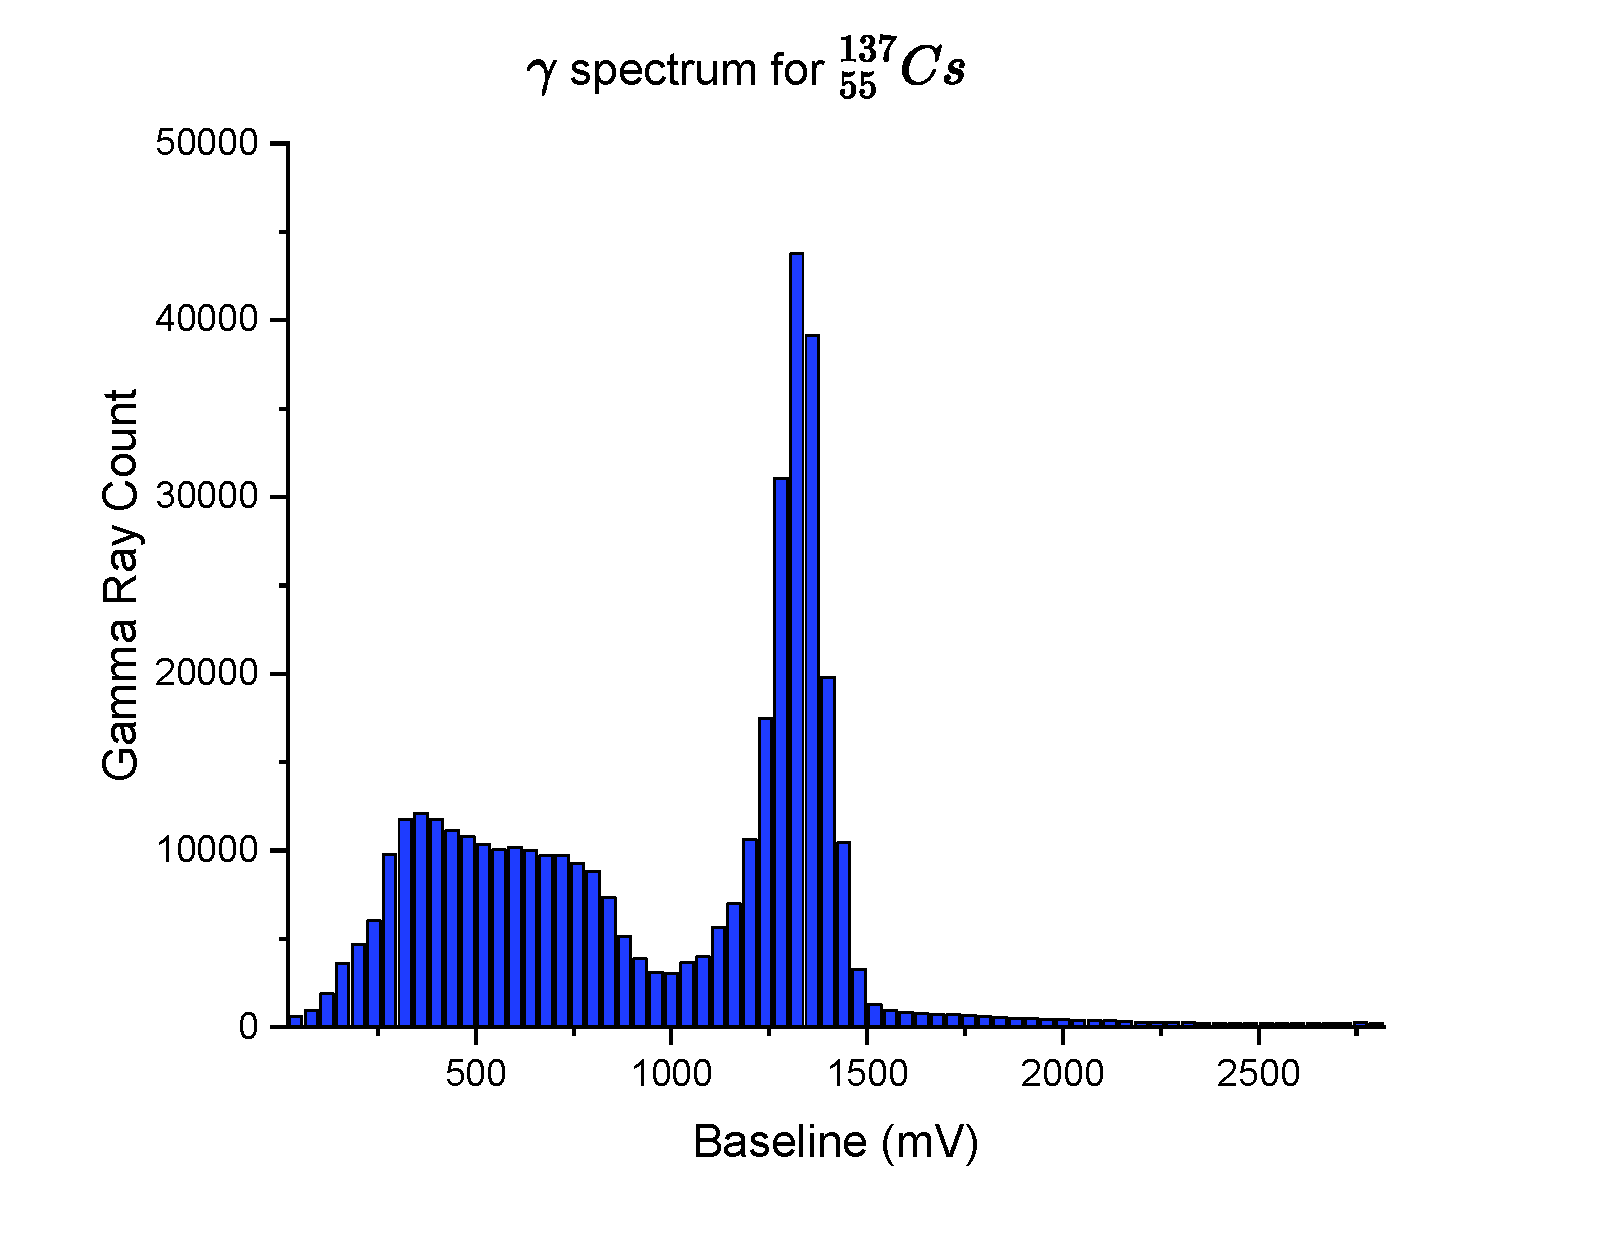
\includegraphics[width=\textwidth]{PH3105_exp3.pdf}
\end{figure}
\end{document}

